\documentclass[12pt]{article}
\usepackage{graphicx}
\title{The Plutonium Blockchain}
\usepackage{setspace}
\doublespacing
\usepackage[margin=1.5in]{geometry}
\begin{document}
\pagenumbering{gobble}
\begin{titlepage}
	\begin{center}
		\vspace{1cm}
		\Huge
		\textbf{The Plutonium Blockchain\\}
		\vspace{1.5cm}
		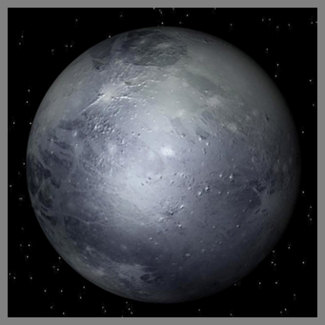
\includegraphics[width=0.4\textwidth]{pluto}\\
		\vspace{1.5cm}
		\large
		Franklin\\
		Franklin High School\\
		218 Oak Street\\
		Franklin, MA, 02038\\
		\vspace{1.5cm}
		\textbf{Sidhartha Chaganti and Michael Gallo}\\
		December 12, 2017
	\end{center}
\end{titlepage}
\newpage
\tableofcontents
\newpage
\pagenumbering{arabic}
\section{Executive Summary}
A peer-to-peer infrastructure that would recreate the financial, corporate, and technological industries of the modern world by removing middleman and their systems and adding security, freedom, and transparency.

Sounds a lot like Bitcoin, right? Fear not, because the Plutonium Blockchain aims to recreate more than the financial industry.

Our current world is plagued by billions of skeptical organisms: humans. Over thousands of years of evolution, the human mind has learned to distrust others. Through first rudimentary consequences and then complex institutions, we have managed to make others more trusting of us. As our communication expands, however, we lack effective communication, and exchanging value requires days or even weeks before the value has finally transferred.

The Blockchain is an emerging technology that makes transactions secure and fast without a middleman. Most adopters, however, only see the Blockchain as a cash-replacement. The fact is, the blockchain protocol has limitless potential.

Frankly, the blockchain can store both assets and transactions; assets are things that users posses. Yes, this can be money, but it can also include your house deed, your license, or your certificate of title for your car. Transactions will transfer assets between two people on the blockchain--when you sell your car to another blockchain user, the buyer will pay you in the form of the currency used on that particular blockchain, and in exchange, you will transfer your certificate of title to that person.

Now, there was no need for a third-party. You didn't have to go to the bank, and the buyer didn't need to pay you through Paypal. It happened on the blockchain, and the transaction would have happened in minutes.

The Blockchain Technology doesn't necessarily have to be limited to consumers; large corporations can take advantage of the speed and security of the blockchain. This is where the Plutonium Blockchain begins its journey.

Russia's geography is one of its greatest strengths. With a surface area larger than that of Pluto, though, Russia faces a large problem economically.

Within this report, we aim to alleviate resource management, economic instability, and political corruption in Russia via the Blockchain. As of 2012, the oil-and-gas sector accounted for 16\% of GDP, 52\% of federal budget revenues, and over 70\% of total exports. Resources play a major role in Russia's economy, and turning the wrong way can lead to major consequences, as seen in 2014, when the Russian economy risked going in to recession due to falling oil prices and sanctions. Furthermore, the Plutonium Blockchain can redistribute political votes to the Russian people. As we will see later, the Blockchain allows for permanent and unalterable votes that can assist in proper elections. The Plutonium Blockchain is aimed to streamline resource management, prevent economic recession, and authenticate Russian politics by making transactions effortless and creating opportunities for cooperation between government and corporations.
\pagebreak
\section{Analysis of the International Business Situation}
\subsection{Trading Country's Economic Structure and Important Economic Information}
This is the ideal time for a massive change to occur to the Russian economy, in late 2016
the country started to come out of an economic recession, and they are still slowly pulling
out. Currently, Russia has one major stock exchange, the Moscow Exchange (MOEX). Our plan is to add the Plutonium Blockchain to this exchange. As of 2016, Russia has \$37.6 million US dollars in inward FDI (foreign direct investments), in 2015 it had merely \$11.8 million (USD) in inward FDI. 
\subsection{Trading Country's Government Structure/Stability}
In theory, Russia's government is headed by an unelected Prime Minister who serves in terms of four years, the Prime Minister is selected by an elected official, the president. The formal title for the Prime Minister is ``Chairman of the Russian Federation''. However, this is not necessarily how it works, for example when you think of the leader of Russia you most likely think of Putin, not Dmitry Medvedev, well Putin is the president of Russia meaning that Medvedev should be in control but for some reason is not. One could say the political situation is very complex. Overall, the Russian Government from the outside (i.e. based on news outlets) seems somewhat unstable, however if you look a little deeper you will find it to be more stable than meets the eye with Putin in charge. What Putin has done as President of the Russian Federation is to try and limit how Russian react to his actions. He monitors protests with a very close eye, this allows him to control the protests and it allows him to show the world how democratic Russia is. Moving on to the foreign trading policy of Russia. Russia’s policy is based off the policies from Australia, the United States, the EU and Chile. Russia uses a CGE model which is a ``\textbf{C}omputable \textbf{G}eneral \textbf{E}quilibrium''. This means that over time, Russia will change how it conducts foreign business based on its import to export ratio for the overall country, not just the specific product, the goal is to maintain an equilibrium for the best possible economic efficiency. Notable, the first word in the CGE model is ``Computable'' this is important because the whole import to export ratio that governs certain aspects of the foreign trade policy is
generated by computers in advance and these can sometimes be wrong causing extremely
unfortunate and expensive issues, including causing unforeseen costs or costs overruns.
\subsection{Laws/Government Agencies}
Currently the United States of America has no laws or regulations that prohibit the use of
non-us online currencies, but the biggest drawback is that not every place is required by law to
accept these currencies, unlike the U.S.D. At this current time, Russia does not have any
regulation around Blockchain technology such as what we will be using. However, much
like the United States, Russia is considering making these currencies regulated on a state
level. At the time of writing no specific details can be found, but it would be an important
fact to keep in mind. 
\subsection{Geographical/Demographic Information}
Russia is the world's largest country by area, but they are \#215 on the world's list in terms
of population density, meaning that their people are spread out over a large area. In terms
of Geography, Russia, if not just because of sheer size, has a little bit of everything,
mountains, rivers, ocean access. Russia being so spread out can make it difficult for things, such as contracts and hard paper currency, to be accessible across the entire surface area. Our smart contracts and online, secure, cryptocurrency will make these items easier to transfer across the country and it will also make it more secure.

\subsection{Analysis of Potential Location/Important Trade Documentation}
The best possible location in Russia for us to base our operations is Russian farm land,
more specifically Ufa Russia. Currently this is farmland, however we plan to turn part of
this 21,755 Acre, \$9.37M (USD) facility into a data center. Data centers do not require
much, only large plots of (preferably cheap) land and power. Speaking of power, it costs
about \$0.10 (USD) per square foot for basic heating/cooling, gas service and other basic
utilities. We should be able to keep it around that price by not having unnecessary things,
such as gas, and getting the most power-efficient servers possible. Russia is the largest
country on Earth w i t h an area of 6.602 million square miles, which is larger than the
surface area of former planet Pluto. This large swath of land is responsible for the
unconquerable quality Russia possesses. While Russia's geography allows for
protection and vast natural resources, it is also one of Russia's great weaknesses.
\pagebreak
\section{Problem}
Russia is the largest country on Earth with an area of 6.602 million square miles, which is larger than the surface area of former planet Pluto. This large swath of land is responsible for the unconquerable quality Russia possesses. While Russia's geography allows for protection and vast natural resources, it is also one of Russia's great weaknesses.

\paragraph{Political Corruption} The majority of Russians live in the European side of the country. This means that the Russian Government (based in Moscow) will be heavily focused on European affairs. However, there is also some corruption within the political scene of Russia, and thus people are not able to express their vote. With the Blockchain, we will introduce a voting system that is anonymous and incorruptible because it is immutable.

\paragraph{Economic Instability} The average GDP per capita of Russia is \$8,748.36. This is half of the GDP per capita that Russia had in 2013. As a result, there is some economic stability that must be fixed. With our Blockchain Technology, we hope to alleviate this problem by introducing a stable currency that reintroduces privacy and establishes freedom.

\paragraph{Resource Management} Russia depends on the exportation of its natural resources for a stable economy. In fact, Russia's natural resources are valued at \$75 trillion U.S. dollars, according to the World Bank. As of 2012, the oil-and-gas sector accounted for 16\% of Russia's GDP, 52\% of federal budget revenues and 70\% of total exports. With the Blockchain Technology, we hope to streamline this process so security is enhanced among corporations and the transaction rate is increased.
\pagebreak
\section{Customer Segments}
Our main demographic will be towards Russians above age 18 (79.06\% or 116 million people living in Russia), although anyone will be able to use it. Specifically, we will be targeting Russians who are in the middle and upper classes. We chose age eighteen because that is the legal voting age in the nation, and one of our main solutions is regarding the political voting system present. Overall, Russians are spending significantly more in 2017, and cryptocurrency is more popular in Russia than in other nations. In addition, we will be targeting businesses related to resource exportation, as they will be the forerunners of using the Blockchain for practical purposes. Lastly, the Blockchain will upgrade the current economic system that uses the Russian ruble, so the service will affect all Russians who use the currency in their daily lives.
\pagebreak
\section{Unique Value Proposition}
People around the world dream about peace, security, and luxury. Our Plutonium Blockchain brings that dream to a reality.

The Blockchain protocol is a fairly young technology, its first practical use being Bitcoin, a cryptocurrency that launched in 2009. Despite its age, the Blockchain protocol will revolutionize the technology industry--and the rest of the world, for that matter. As of December 2017, Bitcoin is valued at \$15,483, and it accounts for 437,125 transactions per day.

So why the Plutonium Blockchain?, you may ask. As of now, cryptocurrencies take advantage of hashing functions that require time and energy to complete, and this results in an exponential difficulty in committing fraud. We aim to take this philosophy and apply it to all areas of improvement, specifically economic instability, resource management, and political corruption.

There have been a multitude of technological revolutions that have changed our very method of thinking. Technology has allowed us do do things we never thought possible before. 

Since the rise of the internet, people around the world have given up on security and identity. We ask them, why must we give up our privacy to be a part of a society?
\pagebreak
\section{Solution}
The Plutonium Blockchain reintroduces freedom and anonymity. With an immutable structure, the Blockchain emphasizes permanence and trust. Lastly, our Blockchain technology will introduce an automated smart contract system that will apply to management systems.
\subsection{Anonymity and Freedom}
The Blockchain operates on a address based system. That means that each person in the Blockchain is an "address", similar to your house or phone number. When someone makes a transaction, they send the money to an address. This means that, on the Blockchain, no one knows who is sending the money and who is getting the money. Since the Blockchain is public and transparent, this "address" feature is very important. Russians will be able to use their money freely without corruption or fraud.
\subsection{Immutability and Permanence}
The Blockchain is a chain of blocks, as the name implies. Each block in the chain contains data about the transaction, and the Blockchain will store this data. Each block contains its own ``hash'' as well as the ``hash'' of the block preceding it. A ``hash'' is a series of numbers and letters derived from a mathematical formula. 
\subsection{Smart Contracts}
A recent addition to the Blockchain Technology is the Smart Contract. Similar to a legal contract, a Smart Contract performs a transaction once the conditions are met. This means businesses need not spend time over fraud and invalid invoices. Within Russia, people will be more trusting of the economy because transactions can become autonomous. This feature is essential to the voting and resource management systems, and Russians will welcome the addition. The Russian Government will allow us to conduct business in a competition with the ruby because it will be a way for Russia, a country not known for technology, to show the world how open it is to allowing technology companies to come in and make advancements in the world.
\pagebreak
\section{Channels}
To accomplish a project of this scale, we have organized different stages of deployment that will eventually lead to a secure, stable, and functioning economy.

Our first stage will be to build the Plutonium Blockchain itself. Then, after testing the Blockchain with a small sample of businesses, we will propose our project to investors, who will hopefully be interested and support our idea.

Second, we will introduce the Blockchain to small and large Russian businesses. This step is crucial because we want create an infrastructure that allows us to expand later. Once our presence is large enough, we plan on incorporating big-time exporting businesses, which will accomplish the resource management stage of our company.

After the Blockchain stabilizes with the increasing number of businesses, we will introduce the system to commercial businesses and to upper class Russians. This way, we will be able to test the Blockchain on a larger scale and make improvements as needed without jeopardizing the Russian economy. As more and more businesses and people use our Blockchain, the value of the currency will increase, and more Russians will want to join the system. This creates a positive feedback loop that is essential to a growing economy. 

Following thorough testing, we will open the Plutonium Blockchain and its currency to every Russian for normal use. We will also require that our business partners prefer using the Pluto currency over others. This creates a dependency that will provide us with leverage for future steps. Once we can identify the Blockchain as ``stable'', we will open the currency to everyone around the world for investments. This establishes a secure economy, which is one of the core solutions.

Last but not least, we plan on introducing the voting system to the Russian government we have gained a foothold in the Russian marketplace, creating a blockchain voting system will allow us to further the expansion of our blockchain by giving us a trustworthy face in the eyes of the Russian people. With such a large dependence, the government will be hard-pressed to refuse the voting system. In addition, we will ask other nations to support our endeavor, should anything go awry. As a monetary incentive, we will offer the Russian government and other governments a substantial amount of Pluto.
\pagebreak
\section{Revenue Streams}
There are many sources of revenue within the Plutonium Blockchain.

Early investors and the creators of the Plutonium Blockchain will be able to invest US Dollars--or any other currency--for Pluto, the currency used for the Plutonium Blockchain, at a fixed price. As people join the blockchain and continue to use the service, the value of each Pluto rises, similar to the stock market.

In addition to early buyers, normal cash-based transactions will undergo a ``gas'' charge that is used to lock the transaction into the blockchain. This charge is rather small, roughly 0.048\% of the transaction itself.

In addition, the Smart Contracts within the Plutonium ecosystem will take a cut from the transaction. However, since there is no middleman, this cut is a third of the 2.9\% cut that Paypal, an online payment system, takes. The Smart Contract fees will be collected by the owners of that particular contract, which could be anyone. This feature will also act as an incentive for future developers.
\pagebreak
\section{Cost Structure}
Due to the nature of the Plutonium Blockchain, the customer acquisition costs decrease as more users join the Blockchain. Since the Plutonium Blockchain is, at its core, a currency, we do not expect to encounter fiscal problems right away. For example, investors will be able to purchase a maximum number of Pluto using US Dollars. For early adopters of the Plutonium Blockchain, we will provide a set number of Pluto for use. Following the early stage, we as a company must advertise our Blockchain to the rest of Russia.

As a company, we will still hire Data Engineers, Software Engineers, Data Analysts, and more. In Russia, the average Cost per Hire (CPH) is \$4,129, and HR budgeting is around 15\% of operational expenses. However, we plan on reducing that HR budget to around 8.5\%. We will achieve this by getting engineers who are just beginning a career and will require fewer benefits than more experienced developers. Although this may seem counter-intuitive, hiring younger developers is actually beneficial. Many experienced developers have developed the secure mindset of ``centralized-coding''--that is, coding for large corporations and governments. As a result, their mindset, while profitable, does not meet the criteria of building a large-scale application. To respond to the ``low-experience'' of young developers, we will be teaching them about Blockchain, and many will have heard of its potential by the time we hire them. For example, Ethereum developer and co-founder Vitalik Buterin was only 19 years old when he coded the Ethereum Blockchain.
\pagebreak
\section{Detailed Financials}
\subsection{Income Statements}
\vspace{1.5cm}
\begin{center}
	Year One Income Statement (USD) \\[1.5ex]
	
	\begin{tabular}{c | c}
	Revenue & \$ -- \\
	Development Costs & \$288,000 \\
	Operational Costs & \$13,000 \\
	Customer Acquisition Costs & \$27,000 \\
	Administrative Costs & \$70,000 \\
	\textbf{Total Costs} & \$398,000 \\
	\textbf{Net Profit} & -\$398,000
	\end{tabular}
\end{center}
\vspace{1.5cm}
\begin{center}
	Year Two Income Statement (USD) \\[1.5ex]
	
	\begin{tabular}{c | c}
	Revenue & \$9,307,500  \\
	Development Costs & \$305,280 \\
	Operational Costs & \$14,780 \\
	Customer Acquisition Costs & \$37,800 \\
	Administrative Costs & \$101,500 \\
	\textbf{Total Costs} & \$458,360 \\
	\textbf{Net Profit} & \$8,849,140
	\end{tabular}
\end{center}
\vspace{1.5cm}
\pagebreak
\begin{center}
	Year Three Income Statement (USD) \\[1.5ex]
	
	\begin{tabular}{c | c}
	Revenue & \$13,036,632 \\
	Development Costs & \$323,596 \\
	Operational Costs & \$14,607 \\
	Customer Acquisition Costs & \$52,920 \\
	Administrative Costs & \$147,175 \\
	\textbf{Total Costs} & \$538,299 \\
	\textbf{Net Profit} & \$12,498,333
	\end{tabular}
\end{center}
\vspace{1.5cm}
\begin{center}
	Year Four Income Statement (USD) \\[1.5ex]
	
	\begin{tabular}{c | c}
	Revenue & \$18,619,892 \\
	Development Costs & \$343,012\\
	Operational Costs & \$15,483 \\
	Customer Acquisition Costs & \$74,088 \\
	Administrative Costs & \$213,404 \\
	\textbf{Total Costs} & \$645,988 \\
	\textbf{Net Profit} & \$17,973,904
	\end{tabular}
\end{center}
\vspace{1.5cm}
\pagebreak
\begin{center}
	Year Five Income Statement (USD) \\%[1.5ex]
	
	\begin{tabular}{c | c}
	Revenue & \$27,171,690 \\
	Development Costs & \$363,593 \\
	Operational Costs & \$16,412 \\
	Customer Acquisition Costs & \$103,723\\
	Administrative Costs & \$309,435 \\
	\textbf{Total Costs} & \$793,164 \\
	\textbf{Net Profit} & \$26,378,526
	\end{tabular}
\end{center}
\begin{center}
	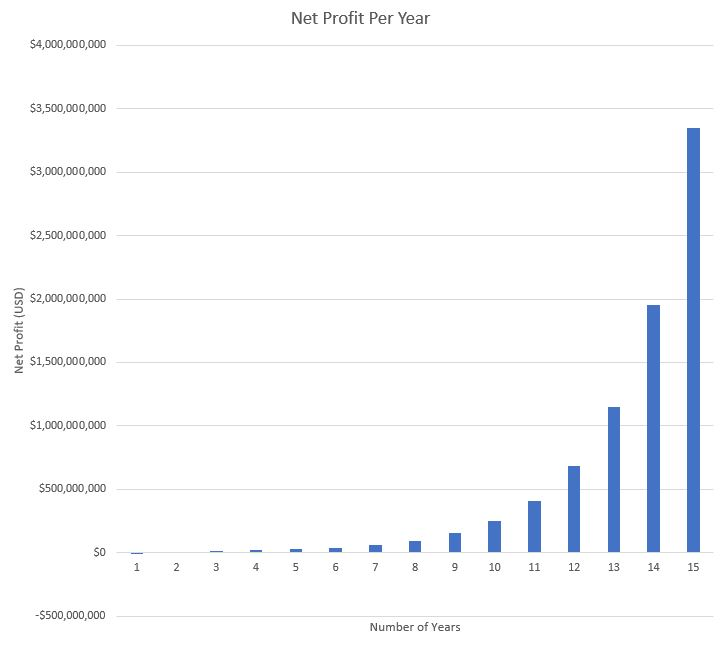
\includegraphics[scale=0.75]{NetProfit}\\
\end{center}
\pagebreak
\subsection{Plan to Meet Capital Needs}
To create the Plutonium Blockchain, our company requires funds for the first year. However, as we gain users and advertise our service to large corporations, our revenue increases dramatically. In fact, we are projected to break one billion dollars in net profit after our thirteenth year of running.

As shown by the numbers and the graph, our revenue is increasing exponentially due to an influx of users every year. However, to get the ball rolling, we will ask private investors who will be able to invest in our company by buying Pluto--the currency of the Blockchain. They will be repaid automatically due to the rising value of Pluto over the coming years. Early adopters will also be given a chance to use our currency in order to gain traction and have a rudimentary source of advertising.
\pagebreak
\section{Key Metrics}
Three key things must be measured; the Number of Daily Transactions (NDT), Number of
Users (NU) and the Value of Daily Transactions (VDT). First, the NDT will give us an
invaluable insight into how often our service is being used, this will give us an idea of how
many businesses accept our new currency (or how useful our business is in terms of the
number of smart contracts). This information will also allow us to make predictions on how
much we need to spend on our increasing need for infrastructure. Next our NU will give us
an idea of how many people those NDT are coming from. This data will allow us to
understand how many transactions a regular person is involved in over the course of a day.
Using this data, we will be able to see how many people use, or believe in, our service.
Finally, is the VDT, which will allow us to understand the value of one day of transactions
and will allow us to predict our overall yearly income as our fee is based on the transaction
total. All the above data is invaluable and will allow us to make predictions and be less
volatile than other, currently existing cryptocurrencies. 
\pagebreak
\section{Competitive Advantage}
Creating a Blockchain is very difficult--a skilled team of developers and analysts is needed. Recreating this team is even more difficult, which means that there will be few competitors that wish to dominate the same market. This results in a very high barrier to entry that prevents most people from recreating our Plutonium Blockchain. Furthermore, companies using our Plutonium Blockchain will be skeptical to use another Blockchain. As a result, only a few blockchains will be dominating in Russia. Our plan is to make the Plutonium Blockchain first prominent in the private sector and infrastructure of Russia so most commerce must flow through our blockchain, deterring future blockchains from capturing the rest of the Russian market. Our currency will also be more predictable than other existing currencies due to its secure and physical nature--the assets and transactions are based on large-scale and physical objects, and since the Plutonium Blockchain will be so ingrained into Russia's infrastructure, our currency will be inherently stable as it revives the Russian economy.
\pagebreak
\section{Conclusion}
The Blockchain technology is very young, and there are many areas that need clarification, both from us, from blockchain experts, and from the world. We admit--cryptocurrencies are a speculative investment. However, that doesn't mean that the underlying technology--blockchain--is speculative.

Due to the nature of the blockchain, it is difficult to obtain accurate numbers. We analyzed the data and presented our balance sheet with the current values. However, it is important to remember that these numbers are subject to change.

To close, we ask you to remember the Great Depression in the 1930s. After the stock market crash, the economic situation in the United States needed change; the United States suffered through 47 previous recessions since its birth. Former president Franklin D. Roosevelt presented his New Deal, which re-imagined the role of the federal government in its economy, and Roosevelt saved capitalism. We may not be Presidents, but we sure can change our world. The Plutonium Blockchain is our ``New Deal''.
\pagebreak
\begin{thebibliography}{10}
\bibitem{worldbank} 
\tiny $"http://Siteresources.worldbank.org/INTRANETTRADE/Resources/WBITraining/London_Conference_Proceedings.Pdf."$ \normalsize \textit{WorldBank.org}, 10 Dec. 2017
 
\bibitem{stats} 
 "List of Countries by Population Density." Countries by Population Density 2015 -
StatisticsTimes.Com, \tiny statisticstimes.com/population/countries-by-population-density.php
 \normalsize
\bibitem{Stratfor} 
Hall, Steven. "Putin's Russia Is More Stable Than It Seems." Stratfor Worldview, Stratfor,
23 Jan. 2016, \tiny worldview.stratfor.com/article/putins-russia-more-stable-it-seems.
\normalsize
\bibitem{Encyclo}
Medvedkov, Olga L., et al. ``Russia.'' Encyclopedia Britannica, Encyclopedia Britannica,
inc., 22 Oct. 2017, \tiny www.britannica.com/place/Russia.
\normalsize
\bibitem{Rus}
``Russian Traditions.'' Russian Traditions, Customs and Rituals,
\tiny www.advantour.com/russia/traditions.htm.
\normalsize
\bibitem{Yfa}
Yfa, Russia land for sale - 21775 acres at LandWatch.Com, \tiny www.landwatch.com/YfaRussia-Farms-and-Ranches-for-sale/pid/200729494.
\normalsize
\bibitem{Net}
Cannucciari, Christopher, and David Guy Levy. Banking on Bitcoin. Banking on Bitcoin,
Netflix, 2016.
\bibitem{peer}
Peer, Chris. “How to Determine a Brand Awareness Budget.” Syncshow - Inbound
Marketing Agency for Manufacturing, \tiny www.syncshow.com/blog/how-to-determine-abrand-awareness-budget.
\normalsize
\bibitem{bridge}
BridgeWest.eu. “Business Start-Up Costs in Russia.” Russia Law Firm oriented towards
foreign investors, \tiny www.lawyersrussia.com/business-start-up-costs-in-russia.
\end{thebibliography}
\end{document}